\section{Methods \& Strategies}

Dynamic Resource Exchange (DRE) is a novel methodology for determing
transactions between suppliers and consumers. The core solution strategy is
agnostic to resource types. Fuel cycle simulation, which is highly dependent on
specific resource properties, i.e., material isotopic vectors, is enabled
through it's agent communication framework. Although it has been designed to
support fuel cycle simulation, the methodology and framework can be adapted to
other complex supply chains.

This section begins by detailing the methodology for querying supply and demand
during the information gathering phase of the DRE in \secref{abm:dre:info}. The
solution phase, in which the defined DRE is translated into a form of the
Multicommodity Transportation Problem (MCTP) and solved, is then described in
\secref{abm:dre:fctp}. 

The DRE has been implemented in the \Cyclus fuel cycle simulator, defining the
key interaction mechanisms for agents. Accordingly, \Cyclus simulations are
described in \secref{results} that showcase novel enabling features. A short
overview of archetypes used in these simulations is provided in
\secref{meth:archs}. Finally, \secref{meth:tariff} describes a new
\texttt{Region} archetype that enables the \textit{in situ} modeling of
interstate trade instruments, such as tariffs.

This section represents the culmination of significant previous effort
\cite{gidden_agent-based_2013, gidden_agent-based_2014,
  gidden_agent-based_slc_2013}. What follows constitutes the refinement of
previous descriptions of the DRE methodology with lessons learned from initial
implementation and usage.

\subsection{Dynamic Resource Exchange}\label{meth:dre}

The DRE enables the constrained transaction of complex resources between
entities in a simulation given a measure of cardinal preference for each
potential transactions. Suppliers and consumers provide information about their
supply and demand during an initial information gathering phase. Complex
constraints can be supplied during this phase. Supply and demand is then
translated into a resource-agnostic \textit{Exchange Graph}. The graph can be
solved feasibly with a heuristic or optimally by translating it into a mixed
integer-linear program. Given a solution, final trades are constructed and
executed.

\subsection{Information Gathering}\label{abm:dre:info}

The DRE begins at any given time step with three \textit{phases}, the
terminology of which is influenced from previous supply chain agent-based
modeling work \cite{julka_agent-based_2002}. Importantly, this
information-gathering step is agnostic as to the supply-demand matching
algorithm used, it is concerned only with querying the current status of supply
and demand in the simulation. The collective information gathering procedure is
shown in Figure \ref{fig:procedure}.

\begin{figure}
  \begin{center}
    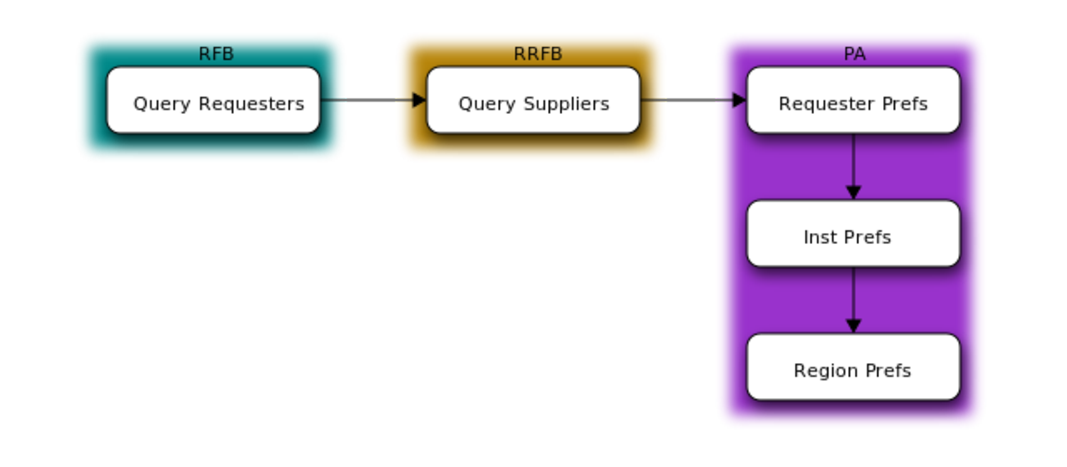
\includegraphics[]{procedure.pdf}
    \caption[]{\label{fig:procedure}
        Schematic illustrating the DRE's information gathering procedure.}
  \end{center}
\end{figure}

The first phase allows consumers of commodities to denote both the quantity of a
commodity they need to consume as well as the target isotopics, or quality, by
\textit{posting} their demand to the market exchange. This posting informs
producers of commodities what is needed by consumers, and is termed the
\textit{Request for Bids} (RFB) phase. Consumers are allowed to over-post, i.e.,
request more quantity than they can actually consume, as long as a corresponding
capacity constraint accompanies this posting. Requests can be denoted as
\textit{exclusive}. An exclusive request is one that must either be met in full
or not at all. Exclusive requests allow the modeling of quantized, packaged
transfers, e.g., fuel assemblies. 

Consumers are allowed to post demand for multiple commodities that may serve to
meet the same combine capacity. For example, consider an LWR that can be filled
with MOX or UOX. It can post a demand for both, but must define a preference
over the set of possible commodities that can be consumed. Such requests are
termed \textit{mutual requests}. Another example is that of an advanced fuel
fabrication facility, i.e., one that fabricates fuel partially from separated
material that has already passed through a reactor. Such a facility can choose
to fill the remaining space in a certain assembly with various types of fertile
material, including depleted uranium from enrichment or reprocessed uranium from
separations. Accordingly, it could demand both commodities as long as it
provides a corresponding constraint with respect to total consumption. A set of
exclusive requests may also be grouped as mutual requests, in which case the set
is termed \textit{mutually exclusive}.

At the completion of the RFB phase, the market exchange will have a set of
request portfolios. Each each portfolio consists of a set requests. Arbitrary
constraints over the set of requests can be provided that are functions of
quantity or quality.  Each request may have an associated preference. For
requests that mutually satisfy a given demand, a preference distribution over
those requests informs the solver as to which should be satisfied first, given
constraints. Finally, each request portfolio has a specific quantity associated
with it.

The second phase allows suppliers to \textit{respond} to the set of request
portfolios, and is termed the \textit{Response to Request for Bids} (RRFB) phase
(analogous to Julka's Reply to Request for Quote phase
\cite{julka_agent-based_2002}). Each request portfolio is comprised of requests
for some set of commodities. Accordingly, for each request, suppliers of that
commodity denote production capacities and an isotopic profile of the commodity
they can provide. Suppliers are allowed to offer the null set of isotopics as
their profile, effectively providing no information. Suppliers are also allowed
to denote responses as exclusive, as is done in the RFB phase. Supply responses
can also be grouped into mutual responses, and sets of responses may be mutually
exclusive. This functionality again supports the notion of quantized orders,
e.g., in the case of fuel assemblies. 

A supplier may have its production constrained by more than one parameter. For
example, a processing facility may have both a throughput constraint (i.e., it
can only process material at a certain rate) and an inventory constraint (i.e.,
it can only hold some total material). Further, the facility could have a
constraint on the quality of material to be processed, e.g., it may be able to
handle a maximum radiotoxicity for any given time step which is a function of
both the quantity of material in processes and the isotopic content of that
material. Multiple of such constraints are allowed. At the completion of the
RRFB phase the possible connections between supplier and producer facilities,
i.e., the arcs in the graph of the transportation problem, have been established
with specific capacity constraints defined both by the quantity and quality of
commodities that will traverse the arcs.

The final phase of the information gathering procedure allows consumer
facilities to adjust their set of preferences and for managers of consumer
facilities to affect the consumer's set of preferences. Accordingly, the last
phase is termed the \textit{Preference Adjustment} (PA) phase. By allowing
facility managers, i.e., a facility's institution and region, to also adjust
preferences, socio-economic models are allowed to inform the exchange of
resources. For example, a region can detect a trans-regional trade between one of
its facilities and a facility in another region. If a tariff model is employed,
the trade preference and be diminished or even removed.

For facilities, preference adjustments occurs in response to the set of
responses provided by producer facilities. Consider the example of a reactor
facility that requests two fuel types, MOX and UOX. It may get two responses to
its request for MOX, each with different isotopic profiles of the MOX that can
be provided. It can then assign preference values over this set of potential MOX
providers. Another prime example is in the case of repositories. A repository
may have a defined preference of material to accept based upon its heat load or
radiotoxicity, both of which are functions of the quality, or isotopics, of a
material. In certain simulators, limits on fuel entering a repository are
imposed based upon the amount of time that has elapsed since the fuel has exited
a reactor, which can be assessed during this phase. The time constraint is, in
actuality, a constraint on heat load or radiotoxicity (one must let enough of
the fission products decay). A repository could analyze possible input fuel
isotopics and set the arc preference of any that violate a given rule to 0,
effectively eliminating that arc.

\subsection{The Nuclear Fuel Cycle Transportation Problem}\label{abm:dre:fctp}

Supply and demand in a nuclear fuel cycle context is inherently a multicommodity
problem. A light water reactor can be fueled by both UOX and MOX fuel, for
instance. How it is fueled is a result both of fuel availability and associated
preferences. Allowing for complex physical and chemical constraints on both
processes and inventories, as well as including economics-based approaches for
determining exchange preferences is a complicated affair. Determining the
optimum solution to such a system is even more complicated. Accordingly,
sophisticated tools in both the operations research and agent based modeling
realms have been leveraged to accomplish the task.

An instance of supply and demand defined by the DRE information gathering step
can be solved in a variety of ways. It can be cast to a constrained, bipartite
network, and any heuristic that provides a feasible solution to such networks
are valid. The system can be solved optimally, however, by formulating the
system as a mathematical program. This section describes a Multicommodity
Transportation Problem variant used for this approach, entitled the
\textit{Nuclear Fuel Cycle Transportation Problem} (NFCTP). A linear program
(LP) formulation and a mixed-integer linear program (MILP) formulation are
provided. A greedy heuristic is also designed and implemented.

The LP formulation can be solved quickly, but allows split orders. In other
words, the LP formulation solves a relaxation of the defined instance that does
not take into account \textit{exclusive} requests or bids. The nuclear fuel
cycle deals with bundled orders, such as nuclear fuel assemblies, thus this
modeling paradigm is only an approximation. The MILP provides a more realistic
exchange, but can take much longer to solve. 

\subsubsection{Terminology}

Objects and data structures generated in the information gathering procedure are
used in the formal definition of the NFCTP. Each portfolio can be considered
separately. The set of supply portfolios is denoted as $S$ and the set of
request portfolios is denoted as $R$, and each agent may have multiple
portfolios in a given exchange. Each supply portfolio is comprised of $s_M$
supply nodes, and each request portfolio is comprised of $r_N$ nodes. The set of
supply nodes is denoted $I$, and the set of request nodes is denoted $J$. The
total number of supply and request nodes is then

\begin{equation}
  \left|{I}\right| = \sum_{s \in S} s_M
\end{equation}

and

\begin{equation}
  \left|{J}\right| = \sum_{r \in R} r_N.
\end{equation}

Each portfolio has a set of commodities, $H$, associated with it. These are
denoted $H_s$ for supply portfolios and $H_r$ for request
portfolios. Furthermore, each portfolio has a set of constraints, $K$,
associated with it. Each constraint has a constraining value, $b_s^k$ and
$b_r^k$, respectively. Additionally, each unique combination of portfolio and
constraint has an associated \textit{constraint coefficient conversion
  function}, denoted $\beta_s^k$ for supply portfolios and $\beta_r^k$ for
request portfolios. Each constraint coefficient conversion function takes as an
argument a proposed resource $q_{i,j}$. Request portfolios are provided a
quantity constraint by default for which coefficients are unity. For a set of
\textit{mutual requests}, $M$, where each request has a request quantity, $x_m$,
the coefficient is defined by the ratio between the the average request quantity
over all mutual requests and $x_m$

\begin{equation}
  \beta_{r, m} = \frac{\bar{x_M}}{x_m}.
\end{equation}

The constraint conversion functions are utilized in the NFCTP by applying them
to the proposed resource transfers, creating constraint
coefficients. Coefficients for supply constraints are defined as

\begin{equation}
  a^k_{i, j} = \beta_s^k(q_{i_j}).
\end{equation}

\noindent
Coefficients for request constraints are defined as

\begin{equation}
  a^k_{j, i} = \beta_r^k(q_{i_j}).
\end{equation}

Finally, for each supply-request node pair, there is an associated preference,
$p_{i, j}$. The set of all preferences is denoted $P$. Similarly, flow between a
node pair is denoted $x_{i, j}$, and the set of all flows is denoted $X$. The
possible flow on an arc is provided an upper bound by the request node quantity,
$\tilde{x_j}$.

\subsubsection{Exchange Graph}

Upon completion of the information gathering phase, a \textit{bipartite} network
is formed. This network is called the \textit{exchange graph}. The network
consists of sending (bid) nodes, $I$, and receiving (request) nodes, $J$. For
each request node, $j$, there may be many bid nodes; however, there is a
one-to-one mapping between bid nodes and request nodes. In other words, a given
bid node, $i$, is a unique response to a request node, $j$. An example of a bare
exchange graph graph is shown in Figure \ref{fig:ex_bare}.

\begin{figure}
  \begin{center}
    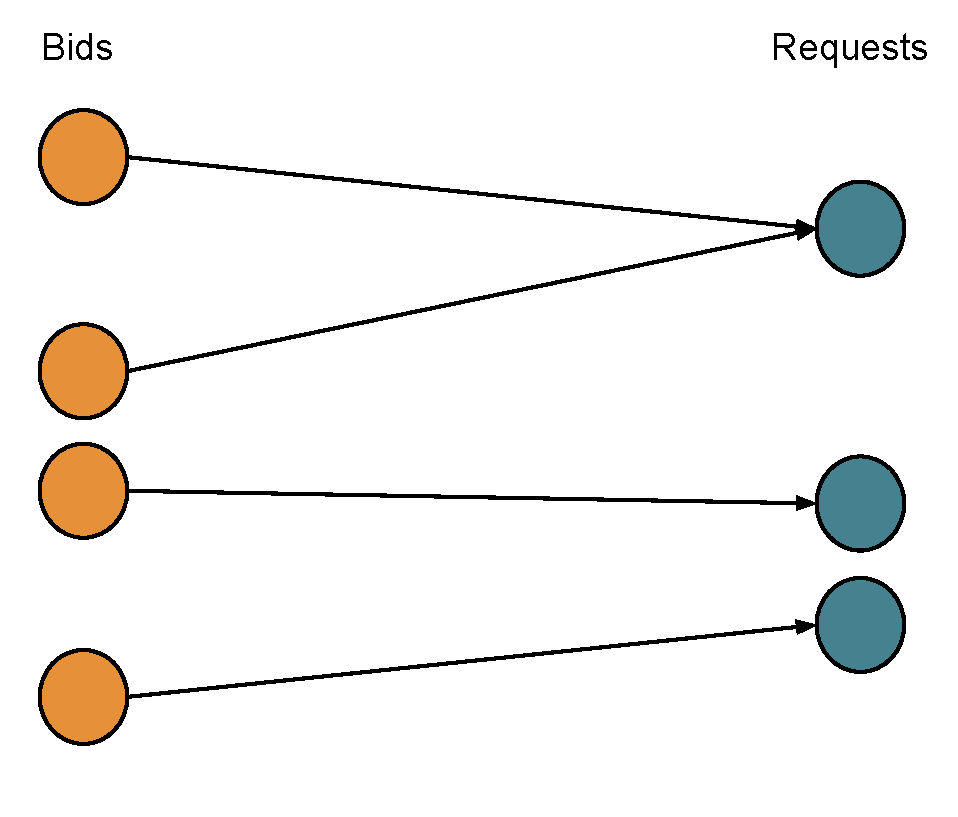
\includegraphics[width=0.75\textwidth]{exchange_bare_words.pdf}
    \caption{A bare example exchange with supply nodes colored orange on left
      and request nodes colored blue on right. As shown, there can be multiple
      supply nodes connected to a request node, but each supply node corresponds
      uniquely to one request node. It is a specific response to that request,
      as outlined in the RRFB phase.}
    \label{fig:ex_bare}
  \end{center}
\end{figure}

In the bipartite graph, portfolios act as partitions that group nodes
together. Node groups share common constraints, and request node groups share a
common notion of satisfiable quantity, i.e., a default mass-based constraint. An
example of a partitioned exchange graph is shown in Figure \ref{fig:ex_groups}.

\begin{figure}
  \begin{center}
    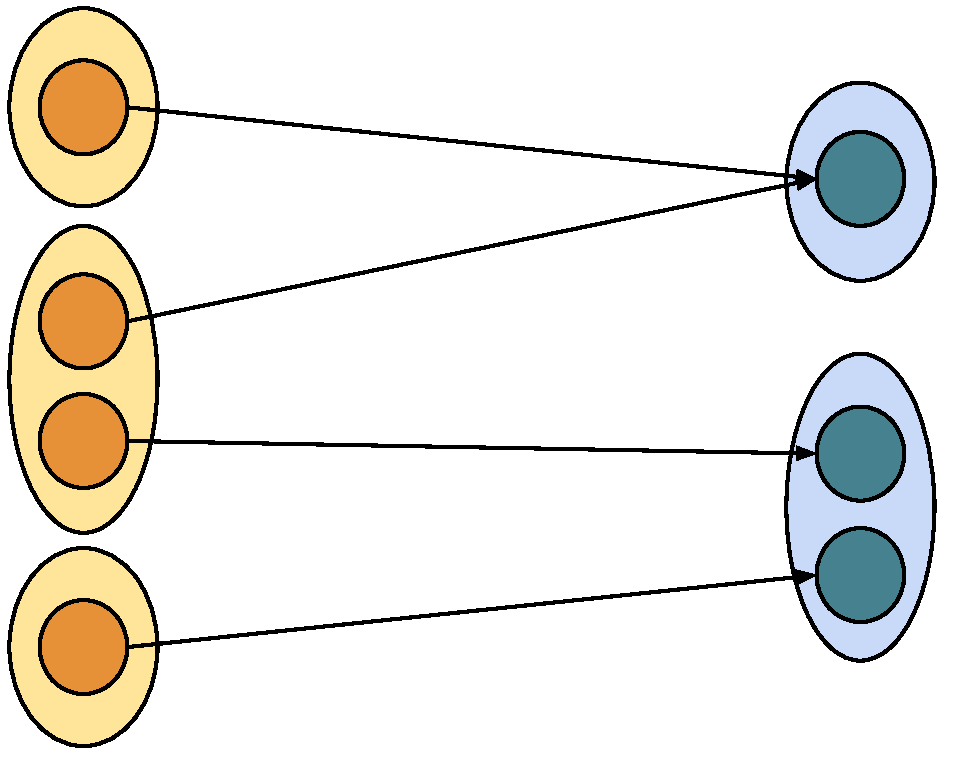
\includegraphics[width=0.75\textwidth]{exchange_groups.pdf}
    \caption{The same exchange shown in Figure \ref{fig:ex_bare} with the
      inclusion of portfolio partitions. In this example, there are three
      supplier agents and two consumer agents. The second consumer has two
      requests (for different commodities) which may satisfy its demand. The
      second supplier can supply the commodities requested by both consumers and
      has provided two bids accordingly.}
    \label{fig:ex_groups}
  \end{center}
\end{figure}

Because of defined constraints, there may not be sufficient supply in the
simulated exchange. To ensure a feasible solution, an unconstrained false supply
node is added to the exchange graph. Additionally, false nodes are added to each
request portfolio and are connected to the false supply source. These arcs are
denoted as \textit{false arcs}. The preferences given to each false arc, $p_f$,
is defined to be lower than the lowest preference in the system, $P$.

\begin{equation}\label{eqn:falsepref}
  p_{f} < \min P
\end{equation}

\noindent
The total number of arcs in the system, $\left|{A_t}\right|$, is then increased
by the number of request portfolios, i.e.,

\begin{equation}
  \left|{A_t}\right| = \left|{A}\right| + \left|{R}\right|
\end{equation}

Because preferences are defined as in Equation \ref{eqn:falsepref}, any false
arc will only be engaged if no other possible arc can be engage, due to capacity
constraints. If any flow is assigned to false arcs after the exchange graph is
solved, that flow is ignored when initiating transactions. Figure
\ref{fig:ex_false} shows a fully defined exchange graph.

\begin{figure}
  \begin{center}
    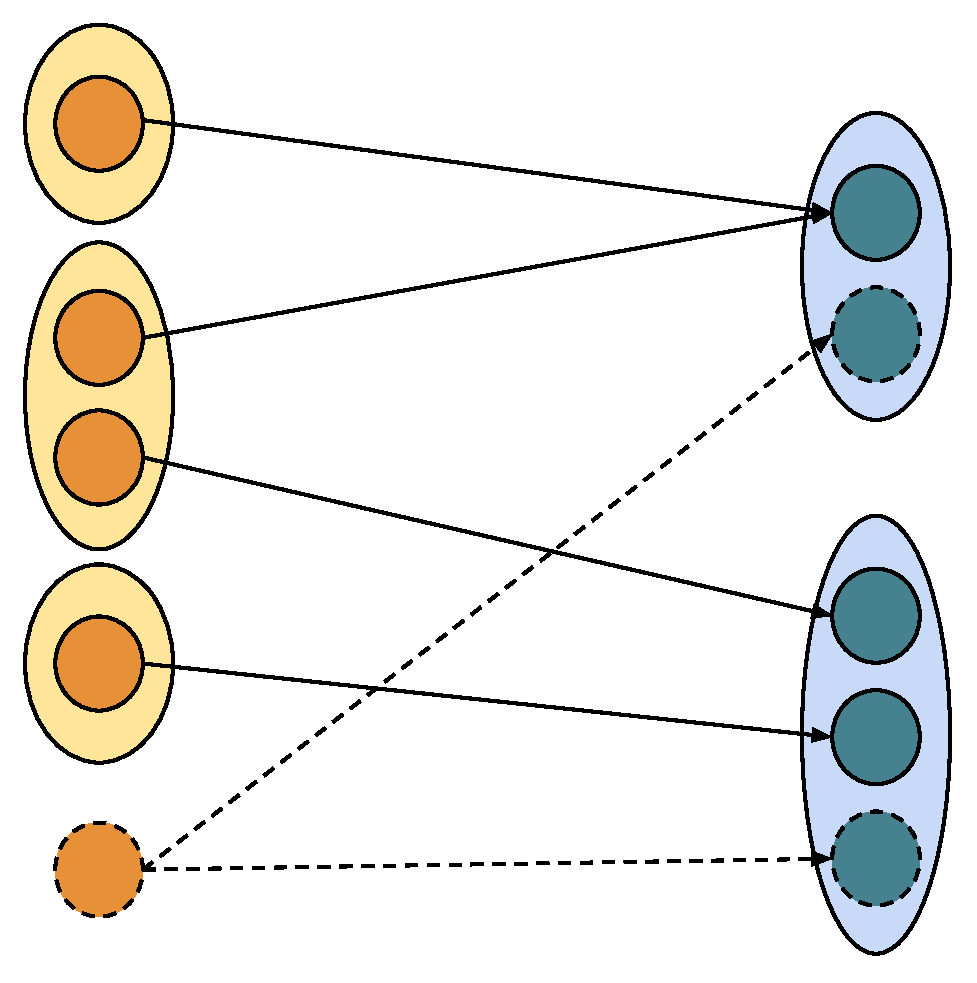
\includegraphics[width=0.75\textwidth]{exchange_false.pdf}
    \caption{The same exchange shown in Figure \ref{fig:ex_groups} with the
      inclusion of false arcs. The false supplier and consumer nodes are shown
      with a dashed outline. Similarly, false arcs are dashed. Note that the
      false nodes have no associated portfolio structure -- there are no
      constraints associated with false nodes and arcs. The inclusion of a false
      supplier and consumer guarantees a feasible solution.}
    \label{fig:ex_false}
  \end{center}
\end{figure}

\subsubsection{Arc Properties}\label{abm:dre:fctp:arcs}

The result of the DRE is flow determined along arcs, where arcs connect supply
nodes to request nodes. A number of properties are defined on arcs, namely
commodities, constraint coefficients, and preferences.

\paragraph{Commodities}

During the information gathering step in \secref{abm:dre:info}, consumers and
suppliers are queried based on \textit{commodities}. A consumer is allowed to
request multiple commodities, and a supplier is allowed to supply multiple
commodities. However, each possible resource transfer, i.e., each arc, is based
on a single commodity. Accordingly, it is possible to color each arc, given a
commodity-to-color mapping.

For example, consider an exchange similar to that shown in Figure
\ref{fig:ex_groups} with two fuel commodities ($A$, $B$), two requesters ($R_1$,
$R_2$), and two suppliers ($S_1$, $S_2$, $S_3$) in the configuration described
by Tables \ref{tbl:ex_sup} and \ref{tbl:ex_req}.

\begin{table}[h]
\centering
\begin{tabular}{c|c}
Supplier & Commodities \\ \hline
$S_1$             & $A$         \\
$S_2$             & $A$, $B$    \\
$S_3$             & $B$         \\
\end{tabular}
\caption{A mapping from suppliers to commodities supplied.}
\label{tbl:ex_sup}
\end{table}

\begin{table}[h]
\centering
\begin{tabular}{c|c}
Consumer & Commodities \\ \hline
$R_1$             & $A$         \\
$R_2$             & $B$        
\end{tabular}
\caption{A mapping from requesters to commodities requested.}
\label{tbl:ex_req}
\end{table}

Given the color map $A$: green, $B$: brown, the resulting exchange
graph can be colored as shown in Figure \ref{fig:ex_groups_color}.

\begin{figure}
  \begin{center}
    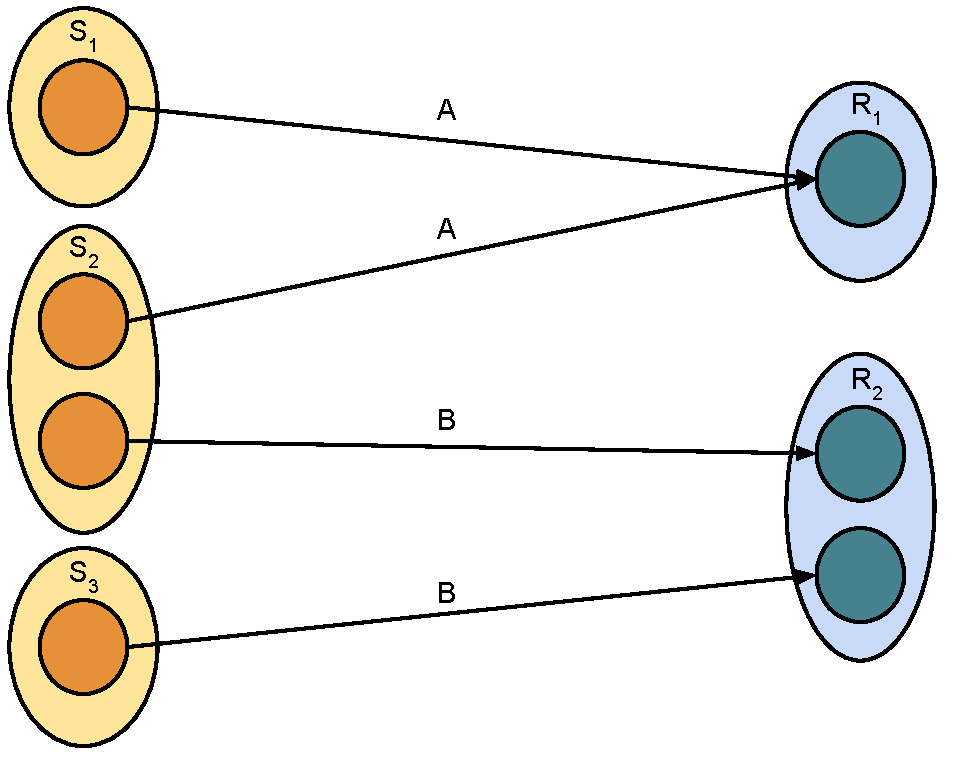
\includegraphics[width=0.75\textwidth]{exchange_groups_color.pdf}
    \caption{The same exchange shown in Figure \ref{fig:ex_groups} arcs colored
      by commodity based on Tables \ref{tbl:ex_sup} and \ref{tbl:ex_req}. A green
      arc corresponds to commodity $A$; a brown arc corresponds to commodity
      $B$.}
    \label{fig:ex_groups_color}
  \end{center}
\end{figure}

The notion of commodities is critical during the information gathering step as
it is the basic classification used in communicating supply and demand. It is
also useful when an exchange graph is formed, because the graph may be able to
be partitioned by collections of commodities. However, once minimally connected
exchange graphs are established, solution mechanisms do not employ the notion of
commodities. Rather, quantities, constraints, and preferences are used.

\paragraph{Constraint Coefficients}

Constraint coefficients are determined for an arc based on the proposed resource
to be transferred along that arc, the requester's constraint conversion
functions, and the suppliers constraint conversion function. An example of
supply-based constraints is provided to help clarify its purpose.

Consider a supplier enrichment facility, $s$, which produces the commodity
enriched uranium (EU). This facility has two constraints on its operation for
any given time period: the amount of Separative Work Units (SWU) that it can
process, $b_{s}^{SWU}$, and the total natural uranium (NU) feed it has on hand.,
$b_{s}^{NU}$. The constraint set for $s$ is then
 
\begin{equation}\label{eqs:enr-constr-commods}
  K_{s} = \{ \mbox{SWU}, \mbox{NU} \}.
\end{equation}

Note that neither of these capacities are measure directly in the units of the
commodity it produces, i.e., kilograms of EU.

Consider a set of requests for enriched uranium that this facility can possibly
meet. Such requests have, in general, two parameters: $P_{j}$, the total product
quantity (in kilograms), and $\varepsilon_{j}$, the product enrichment (in w/o
\nucl{235}{U}).\footnote{The notation for enrichment, $\varepsilon_{j}$, is
  chosen over its normal form, $x_p$, to limit confusion with the notation of
  material flow, $x^h_{i,j}$.}  For the purposes of this constraint set, the
quality of material in question is its enrichment, i.e.,

\begin{equation}\label{eqs:enr-q-swu}
  q_{j} \equiv \varepsilon_{j}.
\end{equation}

These values are set during a prior phase of the overall matching algorithm, and
can therefore be considered constant. Further, note that, in general, an
enrichment facility's operation, or rather its capacity, is governed by two
parameters: $\varepsilon_{f}$, the fraction of \nucl{235}{U} in its feed
material, and $\varepsilon_{t}$, the fraction of \nucl{235}{U} in its tails
material. These parameters determine the amount of SWU required to produce some
amount of enriched uranium, shown in Equation \ref{eqs:swu} as well as the
amount of natural uranium, or feed, required, as shown in Equation \ref{eqs:nu}.

\begin{align}
\begin{split}
\label{eqs:swu}
SWU = & \:\: P ( V(\varepsilon_{j}) 
      + \frac{\varepsilon_{j} - \varepsilon_{f}}
               {\varepsilon_{f} - \varepsilon_{t}} V(\varepsilon_{t}) \\
      & - \frac{\varepsilon_{j} - \varepsilon_{t}}
               {\varepsilon_{f} - \varepsilon_{t}} V(\varepsilon_{f}) )
\end{split}
\end{align}

\begin{equation}
\label{eqs:nu}
F = P \frac{\varepsilon_{j} - \varepsilon_{t}}
           {\varepsilon_{f} - \varepsilon_{t}}
\end{equation}

\noindent
$P$ in Equations \ref{eqs:swu} and \ref{eqs:nu} is the amount of produced
enriched uranium, $F$ is the amount of feed, or natural uranium, and $V(x)$ is
the value function,

\begin{equation}\label{eqs:value}
  V(x) = (1-2x) \ln \left(\frac{1-x}{x}\right)
\end{equation}

Utilizing the above equations, one can denote the functional forms of the
arguments of this facility's two capacity constraints.

\begin{align}
\label{eqs:enr-prod-beta}
\beta_{s}^{NU}(\varepsilon_{j}) = & \:\: \frac{\varepsilon_{j} - \varepsilon_{t}}
                                      {\varepsilon_{f} - \varepsilon_{t}} \\
\begin{split}
\label{eqs:enr-swu-beta}
\beta_{s}^{SWU}(\varepsilon_{j}) = & \:\: V(\varepsilon_{j}) \\
                         & + \frac{\varepsilon_{j} - \varepsilon_{f}}
                                  {\varepsilon_{f} - \varepsilon_{t}} V(\varepsilon_{t}) \\
                         & - \frac{\varepsilon_{j} - \varepsilon_{t}}
                                  {\varepsilon_{f} - \varepsilon_{t}} V(\varepsilon_{f})
\end{split}
\end{align}

These constraints correspond to the per-unit requirements for enriched uranium
of natural uranium feed and SWU. Finally, we can form the set of constraint
equations for the enrichment facility by combining Equations
\ref{eqs:enr-q-swu}, \ref{eqs:enr-prod-beta}, and \ref{eqs:enr-swu-beta}.

\begin{align}
\label{eqs:enr-prod-constr}
\sum_{j \in J}\beta_{s}^{NU}(\varepsilon_{j}) \: x_{s,j}  & \leq b_{s}^{NU} \\
\label{eqs:enr-swu-constr}
\sum_{j \in J}\beta_{s}^{SWU}(\varepsilon_{j}) \: x_{s,j} & \leq b_{s}^{SWU}
\end{align}

\paragraph{Preferences \& Costs}

In any network flow problem, of which transportation problems are a subset, the
objective coefficients associated with transporting commodities is what drives
the solution. Given the nature of supply and demand constraints, the
transportation problem naturally lends itself to a minimum cost formulation. A
preference-based formulation has been presented thus far due to the difficulties
of employing reasonable cost coefficients, as was discussed in 
\secref{intro:prefs}. While directly using costs should be available to users, in
practice using a more abstract notion of preferences is simpler.

Formally, a preference function, $p_{i, j}(h)$, is defined which is a cardinal
preference ordering over a consumer's satisfying commodity set.
 
\begin{equation}
p_{i, j}(h) \:\: \forall i \in I  \:\: \forall h \in H_{r} 
\end{equation}

\noindent
A preference is assigned to each arc in the NFCTP, and are a function both of
the consumer, $j$, and producer, $i$, and the proposed resource transfer from
consumer to producer. The dependence on producer encapsulates the relationship
effects due to managerial preferences. The preference set used in the NFCTP
formulation follows directly from the Preference Adjustment phase described in
\secref{abm:dre:info}.

The notion of a preference is a positive one, that is, an optimal solution
maximizes the product of preference and flow in the system. However, the
transportation problem requires a cost-based objective function. Because
preferences are a proxy for cost and there is a desire to support cost-based
DREs in the future, a preference-to-cost translation function is utilized. A
cost translation function, $f$, is defined that operates on the commodity
preference function to produce an appropriate cost for the NFCTP.

\begin{equation}
f : p_{i,j}(h) \to c_{i,j}
\end{equation}

\noindent
For the purposes of this work, any operator that preserves the preference
monotonicity and cardinal ordering is suitable.  The inversion operator has been
chosen because it preserves required features and also allows for easy
translation from preference to cost as well as translation from cost to
preference.

\begin{equation}
f(x) = \frac{1}{x}
\end{equation}

If cost data and a valid cost assignment methodology is developed in the future,
costs may be used directly, and the preference-to-cost translation may be
ignored.

\subsubsection{Linear Programming Formulation}\label{abm:dre:lp}

Combining the previous discussions, the LP Formulation of the NFCTP, denoted the
NFCTP-LP, can be constructed. In general, the NFCTP is a minimum cost
transportation problem that includes custom constraints as described in previous
sections. Including all of the discussion in the previous sections, the
formulation is straightforward and shown in Equation \ref{eqs:NFCTP-LP}.

%%% 
\begin{subequations}\label{eqs:NFCTP-LP}
  \begin{align}
    %%
    \min_{x} \:\: 
    & 
    z = \sum_{i \in I}\sum_{j \in J}c_{i,j} x_{i,j} 
    & 
    \label{eqs:NFCTP-LP_obj} \\
    %%
    \text{s.t.} \:\: 
    &
    \sum_{i \in I_s} \sum_{j \in J} a^k_{i,j} x_{i,j} \leq b^k_s 
    &
    \: 
    \forall \: k \in K_s, 
    \forall \: s \in S 
    \label{eqs:NFCTP-LP_sup} \\
    %%
    &
    \sum_{j \in J_r} \sum_{i \in I} a^k_{i,j} x_{i,j} \geq b^k_r 
    &
    \: 
    \forall \: k \in K_r,  
    \forall \: r \in R 
    \label{eqs:NFCTP-LP_req} \\
    %%
    &
    x_{i,j} \in [0, \tilde{x_j}]
    &
    \forall \: i \in I, 
    \forall \: j \in J 
    \label{eqs:NFCTP-LP_x}
    %%
  \end{align}
\end{subequations}
%%% 

The variables and sets used to define Equation \ref{eqs:NFCTP-LP} have been
described in detail in previous sections. A short synopsis of the sets used is
provided in Table \ref{tbl:NFCTP-LP-sets}, and a corresponding synopsis of the
variables used is provided in Table \ref{tbl:NFCTP-LP-vars}.

%%% 
\begin{table} [h!]
\centering
\begin{tabularx}{\columnwidth-10pt}{|c|X|} % line wraps second column if too long
\hline
Set         & Description \\
\hline
$S$     & suppliers \\
$R$     & requesters \\
$I$     & all supply nodes \\
$I_s$   & nodes for a supplier $s$ \\
$J$     & all request nodes \\
$J_r$   & nodes for a requester $r$ \\
$K_s$   & constraints for a supplier $s$ \\
$K_r$   & constraints for a requester $r$ \\
$X$         & the feasible set of flows between producers and consumers  \\
\hline
\end{tabularx}
\caption{Sets Appearing in the NFCTP-LP Formulation}
\label{tbl:NFCTP-LP-sets}
\end{table}
%%% 

%%% 
\begin{table} [h!]
\centering
\begin{tabularx}{\columnwidth-10pt}{|c|X|} % line wraps second column if too long
\hline
Variable    & Description \\
\hline
$c_{i,j}$             & the unit cost of flow
                          from producer node $i$ to consumer node $j$  \\
$x_{i,j}$             & a decision variable, the flow 
                          from producer node $i$ to consumer node $j$  \\
$a_{i,j}^k$ & the constraint coefficient for constraint $k$ 
                          on flow between nodes $i$ and $j$  \\
$b_s^k$   & the constraining value for constraint $k$ of supplier $s$ \\
$b_r^k$   & the constraining value for constraint $k$ of requester $r$ \\
$\tilde{x_j}$ & the requested quantity associated with request node $j$ \\
\hline
\end{tabularx}
\caption{Variables Appearing in the NFCTP-LP Formulation}
\label{tbl:NFCTP-LP-vars}
\end{table}
%%%

Notably, a feasible solution to the formulation provided in Equation
\ref{eqs:NFCTP-LP} is guaranteed due to the presence of false arcs. Accordingly,
the DRE using this formulation will never fail within a simulation.

\subsubsection{Mixed Integer Linear Programming Formulation}\label{abm:dre:milp}

The previous linear program (LP) formulation of the Generic Fuel Cycle
Transportation Problem fully describes many of the types of transactions that
arise at any given time step. However, it does not allow the critical case of
reactor fuel orders, which comprise a large amount of material orders within the
simulation context. Specifically, it allows reactor fuel orders to be met by
more than one supplier with an arbitrary amount of the order met by each
supplier. Put another way, the LP formulation does not contain the discrete
material information required to model the transaction of fuel assemblies. 

In order to provide this capability of quantizing orders, binary decision
variables must be introduced. The addition of integer variables changes both the
complexity of the formulation and the complexity of the solution technique. Such
a change requires a Mixed Integer-Linear Program (MILP) formulation and solution
via the branch-and-bound method which solves NP-Hard combinatorial optimization
problems.

\paragraph{Binary Variables}

The primary difference between the LP and MILP formulations is the inclusion
binary decision variables $y_{i,j}$. A variable $y_{i,j}$ has a value of 1 if
flow occurs between producer node $i$ and consumer node $j$. If flow occurs, its
quantity will be equal to the equivalent flow upper bound along that arc,
$\tilde{x}_{j}$, which denote the quantity of a quantized order.

Binary variables, representing quantized flow, are directly related to the
notion of \textit{exclusive} bids and requests discussed in 
\secref{abm:dre:info}. In the MILP formulation, an arc $(i, j)$ is considered
exclusive if either node $i$ or node $j$ was defined as exclusive in the
information gathering phase of the DRE. Accordingly, it is useful to partition
all arcs based on this characteristic. Given the set of arcs $A$, a partition
exists such that $A$ can be separated into exclusive arcs, $A_e$, and
non-exclusive arcs, or arcs that allow partial flow, $A_p$.

\begin{equation}\label{eqs:arc-union}
  A = A_{p} \cup A_{e}
\end{equation}

Similarly, each partition can be further subdivided into partitions based on
supplier and requester. 

\begin{equation}\label{eqs:arc-union}
  A = \bigcup_{r \in R} A_{p_r} \cup A_{e_r}
\end{equation}

\begin{equation}\label{eqs:arc-union}
  A = \bigcup_{s \in S} A_{p_s} \cup A_{e_s}
\end{equation}

\paragraph{Mutually Exclusive Constraints}

\textit{Mutual} requests and responses were described in 
\secref{abm:dre:info}. These are defined as a set of requests or responses, of
which only one may be satisfied. This is represented in the formulation as a
constraint on the associated variables. Again, if a variable $y_{i,j}$ is set to
$1$, flow is sent along arc $(i, j)$. If it is $0$, no flow occurs. A
\textit{mutually exclusive} constraint simply says that only one arc in a mutual
set may have a value of 1.

The set of mutually satisfying arcs is denoted $M_s$ and $M_r$ for suppliers and
requesters, respectively. The associated constraints are then defined by
Equations \ref{eqs:mutual_sup} and \ref{eqs:mutual_req}.

\begin{equation}\label{eqs:mutual_sup}
  \sum_{(i, j) \in M_{s}} y_{i,j} \leq 1 \: \forall \: s \in S 
\end{equation}

\begin{equation}\label{eqs:mutual_req}
  \sum_{(i, j) \in M_{r}} y_{i,j} \leq 1 \: \forall \: r \in R 
\end{equation}

\paragraph{Formulation}

Using the above arc partition notation allows for a much simpler written
formulation of the MILP that looks quite close to the related LP formulation
shown in Equation \ref{eqs:NFCTP-LP}. The full formulation of the NFCTP is shown
in Equation \ref{eqs:NFCTP}.  The sets and variables involved in Equation
\ref{eqs:NFCTP} are described in Tables \ref{tbl:NFCTP-sets} and
\ref{tbl:NFCTP-vars}.


%%% 
% this could probably be realigned 
\begin{subequations}\label{eqs:NFCTP}
  \begin{align}
    %%
    \min_{x, y} \:\: 
    & 
    z \:\: = 
    \sum_{(i, j) \in A_p} c_{i,j} x_{i,j} 
    \: + 
    \sum_{(i, j) \in A_e} c_{i,j} \tilde{x_j} y_{i,j} 
    & 
    \label{eqs:NFCTP_obj} \\
    %%
    \text{s.t.} \:\: 
    &
    \sum_{(i, j) \in A_{p_s}} a^k_{i,j} x_{i,j}
    \: + 
    \sum_{(i, j) \in A_{e_s}} a^k_{i,j} \tilde{x_j} y_{i,j}
    \leq b^k_s 
    &
    \: 
    \forall \: k \in K_s, 
    \forall \: s \in S 
    \label{eqs:NFCTP_sup} \\
    %%
    &
    \sum_{(i, j) \in M_{s}} y_{i,j} \leq 1 
    &
    \forall \: s \in S 
    \label{eqs:NFCTP_mut_sup} \\
    %%
    &
    \sum_{(i, j) \in A_{p_r}} a^k_{i,j} x_{i,j}
    \: + 
    \sum_{(i, j) \in A_{e_r}} a^k_{i,j} \tilde{x_j} y_{i,j}
    \geq b^k_r 
    &
    \: 
    \forall \: k \in K_r,  
    \forall \: r \in R 
    \label{eqs:NFCTP_req} \\
    %%
    &
    \sum_{(i, j) \in M_{r}} y_{i,j} \leq 1 
    &
    \forall \: r \in R 
    \label{eqs:NFCTP_mut_req} \\
    %%
    &
    x_{i,j} \in [0, \tilde{x_j}]
    &
    \forall \: (i, j) \in A_p
    \label{eqs:NFCTP_x} \\
    %%
    &
    y_{i,j} \in \left\{ 0, 1 \right\}
    &
    \forall \: (i, j) \in A_e
    \label{eqs:NFCTP_y}
    %%
  \end{align}
\end{subequations}
%%% 

%%% 
\begin{table} [h!]
\centering
\begin{tabularx}{\columnwidth-10pt}{|c|X|} % line wraps second column if too long
\hline
Set         & Description \\
\hline
$S$     & suppliers \\
$R$     & requesters \\
$A_p$     & arcs that allow \textit{partial} flows \\
$A_e$     & \textit{exclusive} flow arcs  \\
$A_{p_s}$     & arcs that allow \textit{partial} flows for supplier $s$ \\
$A_{e_s}$     & \textit{exclusive} flow arcs for supplier $s$ \\
$A_{p_p}$     & arcs that allow \textit{partial} flows for requester $r$ \\
$A_{e_p}$     & \textit{exclusive} flow arcs for requester $r$ \\
$M_s$     & arcs $(i, j)$ associated with \textit{mutually exclusive} supply for supplier $s$ \\
$M_r$     & arcs $(i, j)$ associated with \textit{mutually exclusive} requests for requester $r$ \\
$X$         & the feasible set of flows between producers and consumers  \\
$Y$         & the binary variable set of flows between producers and consumers  \\
\hline
\end{tabularx}
\caption{Sets Appearing in the NFCTP Formulation}
\label{tbl:NFCTP-sets}
\end{table}
%%% 

%%% 
\begin{table} [h!]
\centering
\begin{tabularx}{\columnwidth-10pt}{|c|X|} % line wraps second column if too long
\hline
Variable    & Description \\
\hline
$c_{i,j}$             & the unit cost of flow
                          from producer node $i$ to consumer node $j$  \\
$x_{i,j}$             & a decision variable, the flow 
                          from producer node $i$ to consumer node $j$  \\
$y_{i,j}$             & a decision variable, whether flow exists 
                          from producer node $i$ to consumer node $j$  \\
$a_{i,j}^k$ & the constraint coefficient for constraint $k$ 
                          on flow between nodes $i$ and $j$  \\
$b_s^k$   & the constraining value for constraint $k$ of supplier $s$ \\
$b_r^k$   & the constraining value for constraint $k$ of requester $r$ \\
$\tilde{x_j}$ & the requested quantity associated with request node $j$ \\
\hline
\end{tabularx}
\caption{Variables Appearing in the NFCTP Formulation}
\label{tbl:NFCTP-vars}
\end{table}
%%%

The examples of the various constraints from the previous section also apply
here. The only difference is the notion of the binary variables, $y_{i,j}$,
which act as on/off switch as to whether a consumer's entire requested amount of
a resource is met by a supplier or not. 

Using this advanced formulation adds significant complexity to the resolution
method at every time step. However, should a user wish to find a feasible
solution in a shorter amount of time, simple heuristics exist. Such a heuristic
used in Cyclus is provided in \secref{abm:dre:nfctp:heur}, and further heuristic
development is a fruitful area of future work.

Note that each constraint coefficient for binary variables can be rewritten as
Equation \ref{eqs:constr_simple} and each objective coefficient can be rewritten
as Equation \ref{eqs:obj_simple}.

\begin{equation}\label{eqs:constr_simple}
a^{k\prime}_{i,j} = a^k_{i,j} \tilde{x_j}
\end{equation}

\begin{equation}\label{eqs:obj_simple}
c^{\prime}_{i,j} = c_{i,j} \tilde{x_j}
\end{equation}

Using both updated definitions, a simpler formulation can be written and is shown
in Equation \ref{eqs:NFCTP_simp}.

%%% 
% this could probably be realigned 
\begin{subequations}\label{eqs:NFCTP_simp}
  \begin{align}
    %%
    \min_{x, y} \:\: 
    & 
    z \:\: = 
    \sum_{(i, j) \in A_p} c_{i,j} x_{i,j} 
    \: + 
    \sum_{(i, j) \in A_e} c^{\prime}_{i,j} y_{i,j} 
    & 
    \label{eqs:NFCTP_simp_obj} \\
    %%
    \text{s.t.} \:\: 
    &
    \sum_{(i, j) \in A_{p_s}} a^k_{i,j} x_{i,j}
    \: + 
    \sum_{(i, j) \in A_{e_s}} a^{k\prime}_{i,j} y_{i,j}
    \leq b^k_s 
    &
    \: 
    \forall \: k \in K_s, 
    \forall \: s \in S 
    \label{eqs:NFCTP_simp_sup} \\
    %%
    &
    \sum_{(i, j) \in M_{s}} y_{i,j} \leq 1 
    &
    \forall \: s \in S 
    \label{eqs:NFCTP_simp_mut_sup} \\
    %%
    &
    \sum_{(i, j) \in A_{p_r}} a^k_{i,j} x_{i,j}
    \: + 
    \sum_{(i, j) \in A_{e_r}} a^{k\prime}_{i,j} y_{i,j}
    \geq b^k_r 
    &
    \: 
    \forall \: k \in K_r,  
    \forall \: r \in R 
    \label{eqs:NFCTP_simp_req} \\
    %%
    &
    \sum_{(i, j) \in M_{r}} y_{i,j} \leq 1 
    &
    \forall \: r \in R 
    \label{eqs:NFCTP_simp_mut_req} \\
    %%
    &
    x_{i,j} \in [0, \tilde{x_j}]
    &
    \forall \: (i, j) \in A_p
    \label{eqs:NFCTP_simp_x} \\
    %%
    &
    y_{i,j} \in \left\{ 0, 1 \right\}
    &
    \forall \: (i, j) \in A_e
    \label{eqs:NFCTP_simp_y}
    %%
  \end{align}
\end{subequations}
%%% 

\subsubsection{A Heuristic Solution}\label{abm:dre:nfctp:heur}

With full simulation domain knowledge of supply and demand, including false
arcs, a feasible solution can be found. By definition a feasible solution is a
\textit{solution} to the possible flow of resources, but not necessarily an
\textit{optimal} solution. Many heuristics may be applied to bipartite graphs
with constrained flows. A simple \textit{greedy} heuristic is presented here
and implemented. 

The maximum flow along an arc, $x_{max}$, depends on the constraints associated
with each node on the arc. For nodes $i$ and $j$ belonging to portfolios $s$ and
$r$, respectively, the maximum allowable flow is defined as

\begin{equation}
  x_{max} = \min 
        \lbrace 
        \min \lbrace \frac{b^k_s}{a^k_{i, j}} 
        \: \forall k \in K_s \rbrace, 
        \: \min \lbrace \frac{b^k_r}{a^k_{i, j}} 
        \: \forall k \in K_r \rbrace
        \rbrace.
\end{equation}

The Greedy Exchange Heuristic matches maximum flow along arcs, up to the
requested amount defined by each request portfolio, $q_r$, after having sorted
all arcs. The constraining values of each arc, $b_k$, are updated upon
declaration of a match (via an \code{AddMatch} function) in Algorithm
\ref{alg::greedy}.

\begin{algorithm}[!h]
 \SetAlgoLined
 \KwData{A resource exchange graph with constraints and preferences.}
 \KwResult{A valid set of resource flows.}
 sort request partitions by average preference\;
 \ForAll{$r \in R$} {
   sort requests by average preference\;
   matched $\leftarrow$ 0\;        
   \While{matched $\leq q_r$ and $\exists$ a request} {
     get next request\;
     sort incoming arcs by preference\;
     \While{matched $\leq q_r$ and $\exists$ an arc} {
       get next arc\;
       remaining $\leftarrow q_r$ - matched\;
       to\_match $\leftarrow \min \lbrace$remaining, $x_{max} \rbrace$\;
       \code{AddMatch}(arc, to\_match)\;
       matched $\leftarrow$ matched + to\_match\;
     }
   }
 }
 \caption{Greedy Exchange Heuristic}\label{alg::greedy}
\end{algorithm}

\subsubsection{Departure from the MCTP}

The classic MCTP includes the coloring of flows based on commodity type. For
example, for a commodity, $h$, the unit cost of flow would be $c^h_{i,j}$ rather
than $c_{i, j}$. This is included because multiple commodities can flow along
the same arc in the MCTP. In other words, the node-arc incidence matrix includes
an extra commodity dimension. 

The multicommodity nature of the NFCTP is included in constraints, rather than
arcs. Because each node pairing, $(i, j)$, corresponds to a specific, proposed
resource transfer, it can only have one commodity associated with it. Instead,
the constraint set, $K$, is applied over multiple arcs, where each arc is
assigned its own commodity. 

Take the enrichment facility example, expanding on the previous discussion. Note
that an enrichment facility takes feed uranium and then enriches its
\nucl{235}{U} content. This feed uranium can come from different sources which
have different feed enrichments. In practice, the most likely sources of feed
uranium are natural uranium (NU) or recycled uranium (RU), a product of
reprocessing light water reactor fuel. Recycled uranium may be advantageous to
use if it has a higher weight percent of \nucl{235}{U} than does natural
uranium. We can now state the set the values for $H_{r}$ for this facility:

\begin{equation}\label{eqs:enr-dem-commods}
  H_{r} = \{ \mbox{NU}, \mbox{RU} \}
\end{equation}

\noindent
One or more constraints would then accompany any requests. For example, one
could constraint total \nucl{235}{U} content needed, which would include both NU
and RU flows.

\subsection{Implementation}\label{abm:dre:impl}

The DRE and its solution framework are implemented in three layers. The first
layer includes information for specific \code{Resource} types. For example, a
\code{Material}-based exchange is used for agents to communicate supply and
demand information regarding \code{Material} objects. The \textit{resource
  layer} is the point of entry and exit of the DRE framework. It is the
agent-facing interface of the DRE: supply and demand is provided to the DRE as
input during the information gathering step, and trades to be executed are
provided to agents as output.

The second layer, called the \textit{exchange layer}, is a
\code{Resource}-agnostic implementation of a specialized bipartite
graph. Supply/demand constructs in the first layer are translated into stateful
objects representing nodes, arcs, constructs that carry constraint information,
\textit{et cetera}. The collection of objects and structures combine to create
an \code{ExchangeGraph}. Any custom, Cyclus-aware solver can be applied to an
\code{ExchangeGraph} to determine a feasible solution to the DRE.

In order to use sophisticated, 3\textsuperscript{rd} party LP and MILP solving
libraries, the \code{ExchangeGraph} must be translated into an appropriate data
structure representing an instance of the NFCTP, resulting in the
\textit{formulation layer}. The Open Solver Interface (OSI) \cite{coinosi} is
used to create the necessary formulation structures, including a constraint
matrix and objective coefficient vector. The NFCTP instance is then solved.

After a feasible, perhaps optimal, solution to the NFCTP is found, whether in
the exchange or formulation layer, the solution is back-translated to the
resource layer. The agents associated with successful supply-demand connections
are informed, and trades of resources between agents are executed. A graphic of
the entire workflow is shown in Figure \ref{fig:dre_impl}.

\begin{figure}
  \begin{center}
    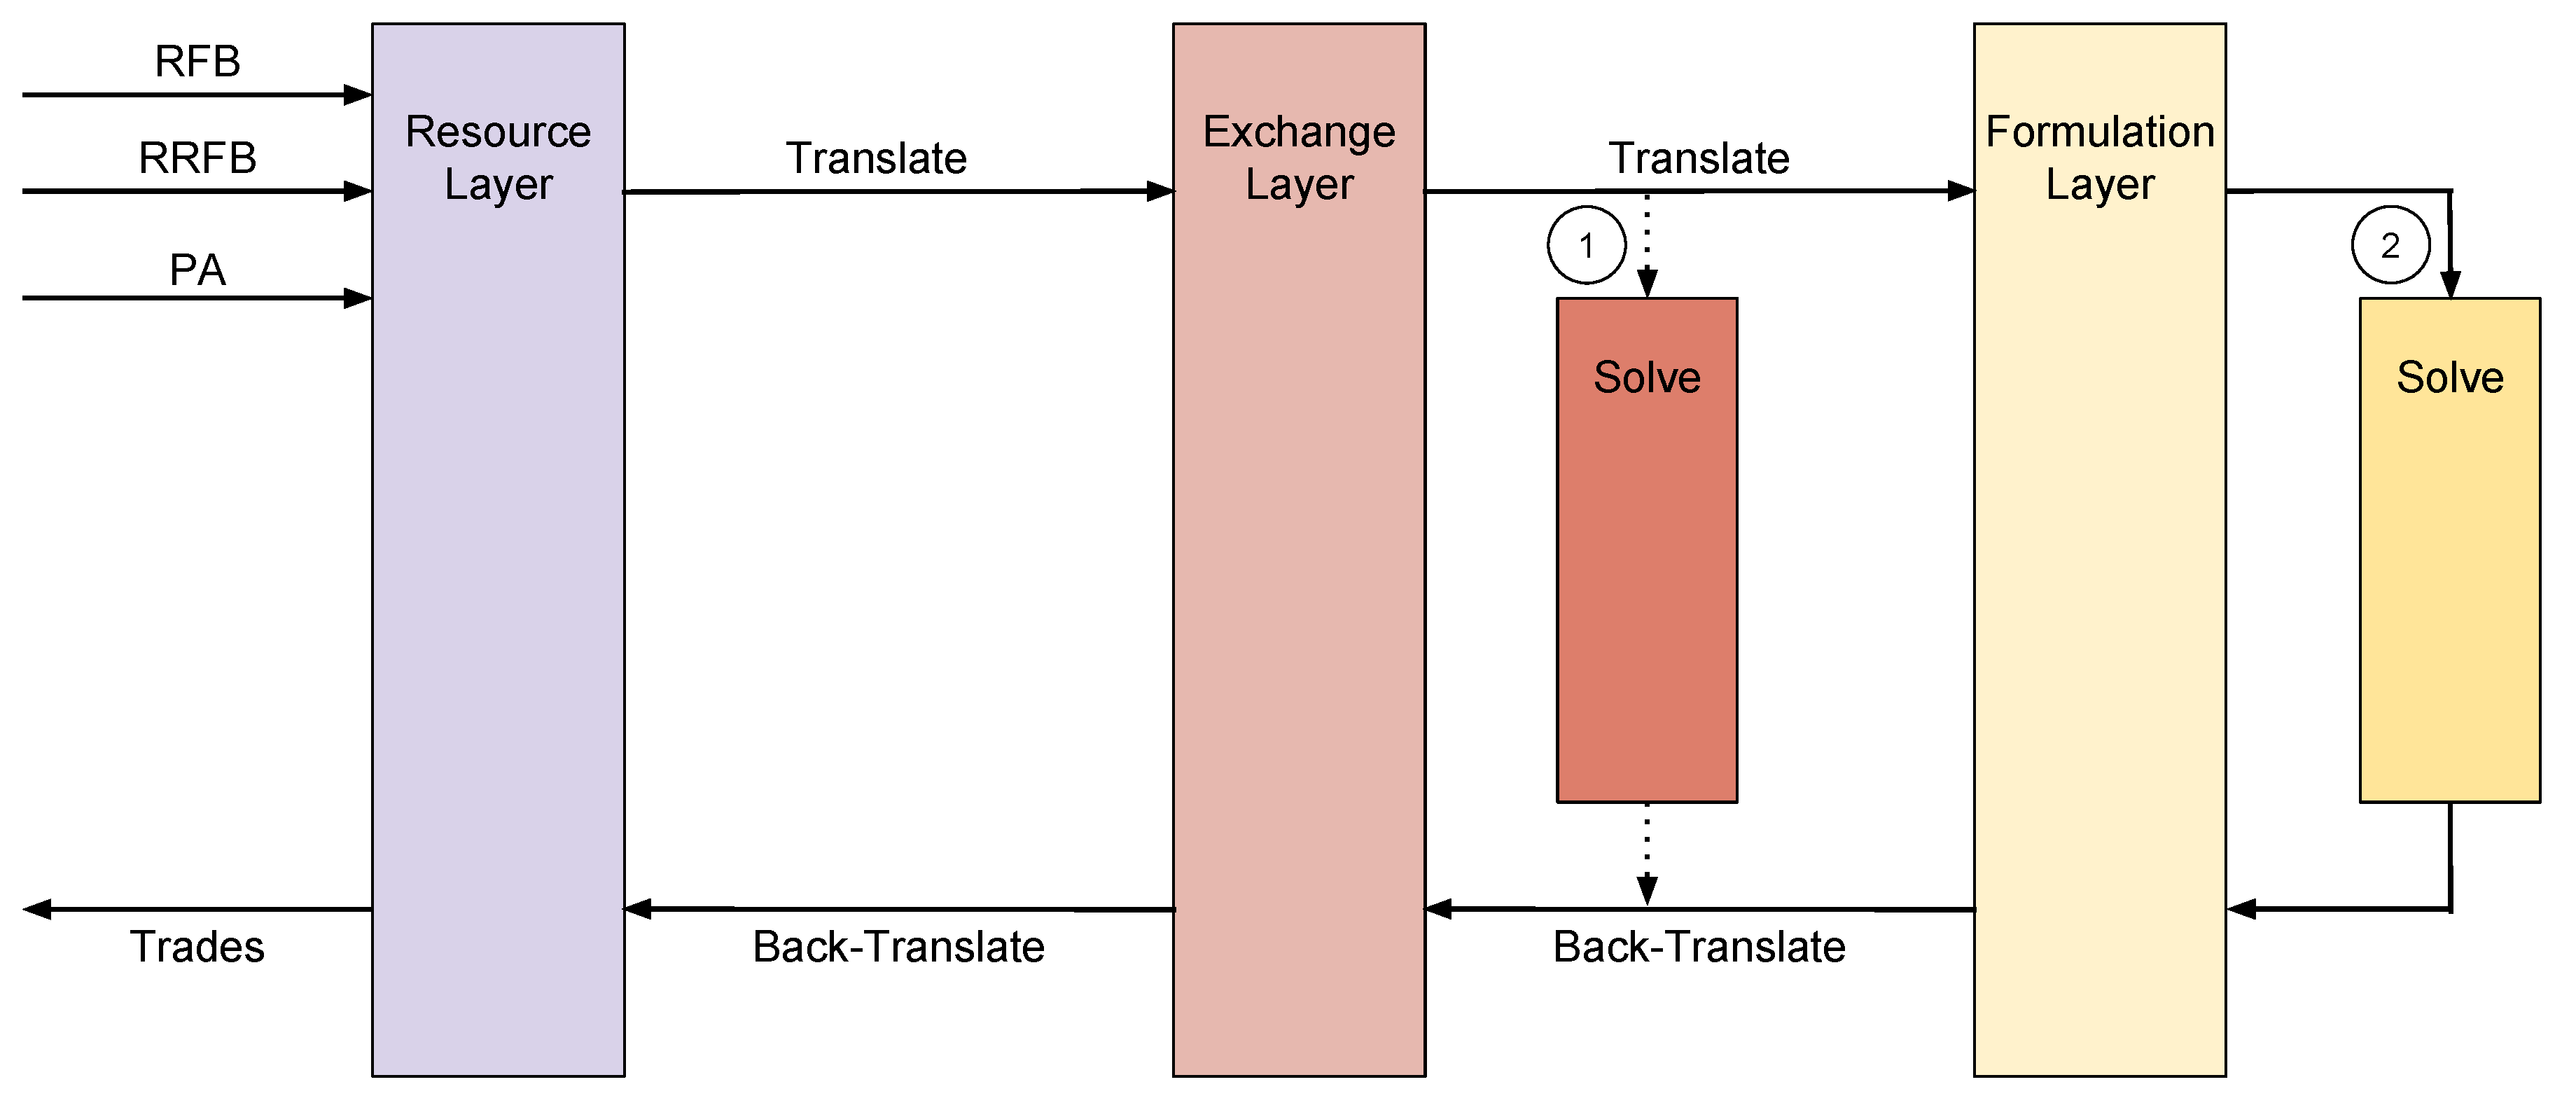
\includegraphics[width=\textwidth]{exchange_xlation.pdf}
    \caption[]{
      \label{fig:dre_impl}
      The full DRE workflow is shown. The information gathering phase results in
      the resource layer. The resource layer is translated to the exchange
      layer; a decision is made whether to continue translation or to directly
      solve, marked by the number $1$. If the exchange is not solved, it is
      translated into an instance of the NFCTP resulting in the formulation
      layer. A choice of solver is made, marked by the number $2$, and the
      instance is solved.  The solution is back-translated through the exchange
      and resource layers. The result is a series of resource trades to be
      executed in the simulation.}
  \end{center}
\end{figure}

\subsubsection{Resource Layer}

The resource layer utilizes \textit{templated} classes in order to reduce the
amount of code required for implementation. Each object is templated on the
concrete \code{Resource} type, e.g., the \code{Material} and \code{Product}
classes. The fundamental data structures in the resource layer reflect the
constructs of the information gathering procedure described in 
\secref{abm:dre:info}.

In the RFB phase of the DRE, agents populate \codeb{Request\-Portfolio}s with
\code{Request}s and \codeb{Capacity\-Constraint}s. A \code{Request}
defines a desired \code{Resource}, communicating quantity, quality, and
preference. Any number of \codeb{Capacity\-Constraint}s may be added to a
\codeb{Request\-Portfolio}. A \codeb{Capacity\-Constraint} defines a
capacitating value and a conversion function that takes as an argument a
\code{Resource} and returns a value in units of the conversion function. For
\codeb{Request\-Portfolio}s, constraints are assumed to be demand
constraints, i.e., take the form of a greater-than constraint. In the RRFB phase
of the DRE, agents populate \codeb{Bid\-Portfolio}s with \code{Bid}s and
\codeb{Capacity\-Constraint}s. Agents can inspect the population of
\code{Request}s and associated \code{Resource}s. A \code{Bid} targets a
specific \code{Request}, responding with a proposed \code{Resource} to
transfer to the requester. \codeb {Capacity\-Constraint}s are applied to all
\code{Bid}s in a portfolio. For bidders, constraints are assumed to be
less-than constraints. Before continuing, requesting agents and their managers
are allowed to alter the preference associated with each
\code{Request}-\code{Bid} pair in the PA phase of the DRE. When a solution
to the DRE is found, bidders associated with successful
\code{Request}-\code{Bid} pairs are informed, and a trade of the bidder's
\code{Resource} is initiated.

Future work can be focused on providing more features to the DRE
implementation. A natural extension of the present work is to support both kinds
of constraints, greater and less-than, in \code{Portfolio} data
structures. Additionally, the PA procedure could use a negotiation model that
involves both suppliers and requesters in order to define a final preference for
an arc. Such an extension would allow for more seamless and natural usage of arc
costs in addition to preferences.

\subsubsection{Exchange Layer} 

The exchange layer is constructed by an \code{ExchangeTranslator} object that
translates the resource layer objects into an instance of an
\code{ExchangeGraph}. Request and bid objects are translated to
\code{ExchangeNode}s, and portfolio objects are translated to
\code{ExchangeGroup}s. Constraint coefficient and preference information is
recorded on \code{ExchangeArc}s, which store a reference to a supply
\code{ExchangeNode} and a demand \code{ExchangeNode}. Finally, constraint values
are stored on the appropriate \code{ExchangeGroup} object.

An \code{ExchangeContext} object is tasked with storing a mapping from
\code{Request} and \code{Bid} objects to their associated
\code{ExchangeNode}. Importantly, the exchange layer does \textit{not} depend on
resource type, i.e., the resource type is abstracted away during
translation. Finally, a general solver can be implemented that operates on the
\code{ExchangeGraph}. A solution to the \code{ExchangeGraph} instance is a
mapping from \code{ExchangeArc}s to flow quantities that does not violate the
provided constraints. After a solution is found, it is back-translated to the
resource layer.

\subsubsection{Formulation Layer}

While a solver may operate on the exchange layer, an instance of an
\code{ExchangeGraph} can be translated fully into the NFCTP. Once in an LP or
MILP form, the DRE instance can be solved by sophisticated 3\textsuperscript{rd}
party libraries. In order to interface with a large number of the possible
solvers, including COIN-OR and CPLEX, the COIN-OR OSI API \cite{coinosi} is
utilized.

The translation from the exchange layer to formulation layer is managed by the
\code{ProgTranslator} class. A variable in the NFCTP is associated with each
\code{ExchangeArc}, with variable bounds set by request values on
\code{ExchangeNode}s; a binary variable is used if the arc is exclusive,
otherwise a linear variable is used. Capacity coefficients and preference values
defined for \code{ExchangeArc}s are translated into an objective coefficient
vector and constraint matrix. The right-hand-side $b$ constraint vector is
determined by \code{ExchangeGroup} constraining values.

A solution to the NFCTP instance is determined by the identified solver,
assigning values to linear and integer variables. Linear variable values map
directly to assigned resource flow quantity. If a binary variable is set to
unity in a solution, the maximum possible flow value is assigned, analogous to
$\tilde{x_j}$ in the NFCTP formulation. The variable-flow value assignment is
then back-translated into an equivalent \code{ExchangeArc}-flow value assignment
by the \code{ProgTranslator}.

%%% Highlight dynamic sim
%%%% - new facilities wont break sim (e.g., adding non-interacting facility, adding recycle-capable reactors in a non-recycle scenario, etc.)
%%%% - flexibility
%%%% - repo accepting multiple waste forms

%% - Cyclus Archetypes
